\documentclass[1p]{elsarticle_modified}
%\bibliographystyle{elsarticle-num}

%\usepackage[colorlinks]{hyperref}
%\usepackage{abbrmath_seonhwa} %\Abb, \Ascr, \Acal ,\Abf, \Afrak
\usepackage{amsfonts}
\usepackage{amssymb}
\usepackage{amsmath}
\usepackage{amsthm}
\usepackage{scalefnt}
\usepackage{amsbsy}
\usepackage{kotex}
\usepackage{caption}
\usepackage{subfig}
\usepackage{color}
\usepackage{graphicx}
\usepackage{xcolor} %% white, black, red, green, blue, cyan, magenta, yellow
\usepackage{float}
\usepackage{setspace}
\usepackage{hyperref}

\usepackage{tikz}
\usetikzlibrary{arrows}

\usepackage{multirow}
\usepackage{array} % fixed length table
\usepackage{hhline}

%%%%%%%%%%%%%%%%%%%%%
\makeatletter
\renewcommand*\env@matrix[1][\arraystretch]{%
	\edef\arraystretch{#1}%
	\hskip -\arraycolsep
	\let\@ifnextchar\new@ifnextchar
	\array{*\c@MaxMatrixCols c}}
\makeatother %https://tex.stackexchange.com/questions/14071/how-can-i-increase-the-line-spacing-in-a-matrix
%%%%%%%%%%%%%%%

\usepackage[normalem]{ulem}

\newcommand{\msout}[1]{\ifmmode\text{\sout{\ensuremath{#1}}}\else\sout{#1}\fi}
%SOURCE: \msout is \stkout macro in https://tex.stackexchange.com/questions/20609/strikeout-in-math-mode

\newcommand{\cancel}[1]{
	\ifmmode
	{\color{red}\msout{#1}}
	\else
	{\color{red}\sout{#1}}
	\fi
}

\newcommand{\add}[1]{
	{\color{blue}\uwave{#1}}
}

\newcommand{\replace}[2]{
	\ifmmode
	{\color{red}\msout{#1}}{\color{blue}\uwave{#2}}
	\else
	{\color{red}\sout{#1}}{\color{blue}\uwave{#2}}
	\fi
}

\newcommand{\Sol}{\mathcal{S}} %segment
\newcommand{\D}{D} %diagram
\newcommand{\A}{\mathcal{A}} %arc


%%%%%%%%%%%%%%%%%%%%%%%%%%%%%5 test

\def\sl{\operatorname{\textup{SL}}(2,\Cbb)}
\def\psl{\operatorname{\textup{PSL}}(2,\Cbb)}
\def\quan{\mkern 1mu \triangleright \mkern 1mu}

\theoremstyle{definition}
\newtheorem{thm}{Theorem}[section]
\newtheorem{prop}[thm]{Proposition}
\newtheorem{lem}[thm]{Lemma}
\newtheorem{ques}[thm]{Question}
\newtheorem{cor}[thm]{Corollary}
\newtheorem{defn}[thm]{Definition}
\newtheorem{exam}[thm]{Example}
\newtheorem{rmk}[thm]{Remark}
\newtheorem{alg}[thm]{Algorithm}

\newcommand{\I}{\sqrt{-1}}
\begin{document}

%\begin{frontmatter}
%
%\title{Boundary parabolic representations of knots up to 8 crossings}
%
%%% Group authors per affiliation:
%\author{Yunhi Cho} 
%\address{Department of Mathematics, University of Seoul, Seoul, Korea}
%\ead{yhcho@uos.ac.kr}
%
%
%\author{Seonhwa Kim} %\fnref{s_kim}}
%\address{Center for Geometry and Physics, Institute for Basic Science, Pohang, 37673, Korea}
%\ead{ryeona17@ibs.re.kr}
%
%\author{Hyuk Kim}
%\address{Department of Mathematical Sciences, Seoul National University, Seoul 08826, Korea}
%\ead{hyukkim@snu.ac.kr}
%
%\author{Seokbeom Yoon}
%\address{Department of Mathematical Sciences, Seoul National University, Seoul, 08826,  Korea}
%\ead{sbyoon15@snu.ac.kr}
%
%\begin{abstract}
%We find all boundary parabolic representation of knots up to 8 crossings.
%
%\end{abstract}
%\begin{keyword}
%    \MSC[2010] 57M25 
%\end{keyword}
%
%\end{frontmatter}

%\linenumbers
%\tableofcontents
%
\newcommand\colored[1]{\textcolor{white}{\rule[-0.35ex]{0.8em}{1.4ex}}\kern-0.8em\color{red} #1}%
%\newcommand\colored[1]{\textcolor{white}{ #1}\kern-2.17ex	\textcolor{white}{ #1}\kern-1.81ex	\textcolor{white}{ #1}\kern-2.15ex\color{red}#1	}

{\Large $\underline{11a_{10}~(K11a_{10})}$}

\setlength{\tabcolsep}{10pt}
\renewcommand{\arraystretch}{1.6}
\vspace{1cm}\begin{tabular}{m{100pt}>{\centering\arraybackslash}m{274pt}}
\multirow{5}{120pt}{
	\centering
	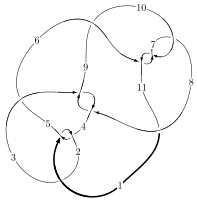
\includegraphics[width=112pt]{../../../GIT/diagram.site/Diagrams/png/259_11a_10.png}\\
\ \ \ A knot diagram\footnotemark}&
\allowdisplaybreaks
\textbf{Linearized knot diagam} \\
\cline{2-2}
 &
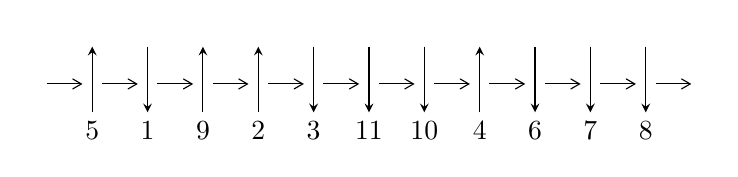
\begin{tikzpicture}[x=20pt, y=17pt]
	% nodes
	\node (C0) at (0, 0) {};
	\node (C1) at (1, 0) {};
	\node (C1U) at (1, +1) {};
	\node (C1D) at (1, -1) {5};

	\node (C2) at (2, 0) {};
	\node (C2U) at (2, +1) {};
	\node (C2D) at (2, -1) {1};

	\node (C3) at (3, 0) {};
	\node (C3U) at (3, +1) {};
	\node (C3D) at (3, -1) {9};

	\node (C4) at (4, 0) {};
	\node (C4U) at (4, +1) {};
	\node (C4D) at (4, -1) {2};

	\node (C5) at (5, 0) {};
	\node (C5U) at (5, +1) {};
	\node (C5D) at (5, -1) {3};

	\node (C6) at (6, 0) {};
	\node (C6U) at (6, +1) {};
	\node (C6D) at (6, -1) {11};

	\node (C7) at (7, 0) {};
	\node (C7U) at (7, +1) {};
	\node (C7D) at (7, -1) {10};

	\node (C8) at (8, 0) {};
	\node (C8U) at (8, +1) {};
	\node (C8D) at (8, -1) {4};

	\node (C9) at (9, 0) {};
	\node (C9U) at (9, +1) {};
	\node (C9D) at (9, -1) {6};

	\node (C10) at (10, 0) {};
	\node (C10U) at (10, +1) {};
	\node (C10D) at (10, -1) {7};

	\node (C11) at (11, 0) {};
	\node (C11U) at (11, +1) {};
	\node (C11D) at (11, -1) {8};
	\node (C12) at (12, 0) {};

	% arrows
	\draw[->,>={angle 60}]
	(C0) edge (C1) (C1) edge (C2) (C2) edge (C3) (C3) edge (C4) (C4) edge (C5) (C5) edge (C6) (C6) edge (C7) (C7) edge (C8) (C8) edge (C9) (C9) edge (C10) (C10) edge (C11) (C11) edge (C12) ;	\draw[->,>=stealth]
	(C1D) edge (C1U) (C2U) edge (C2D) (C3D) edge (C3U) (C4D) edge (C4U) (C5U) edge (C5D) (C6U) edge (C6D) (C7U) edge (C7D) (C8D) edge (C8U) (C9U) edge (C9D) (C10U) edge (C10D) (C11U) edge (C11D) ;
	\end{tikzpicture} \\
\hhline{~~} \\& 
\textbf{Solving Sequence} \\ \cline{2-2} 
 &
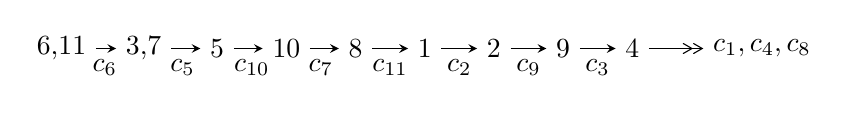
\begin{tikzpicture}[x=25pt, y=7pt]
	% node
	\node (A0) at (-1/8, 0) {6,11};
	\node (A1) at (17/16, 0) {3,7};
	\node (A2) at (17/8, 0) {5};
	\node (A3) at (25/8, 0) {10};
	\node (A4) at (33/8, 0) {8};
	\node (A5) at (41/8, 0) {1};
	\node (A6) at (49/8, 0) {2};
	\node (A7) at (57/8, 0) {9};
	\node (A8) at (65/8, 0) {4};
	\node (C1) at (1/2, -1) {$c_{6}$};
	\node (C2) at (13/8, -1) {$c_{5}$};
	\node (C3) at (21/8, -1) {$c_{10}$};
	\node (C4) at (29/8, -1) {$c_{7}$};
	\node (C5) at (37/8, -1) {$c_{11}$};
	\node (C6) at (45/8, -1) {$c_{2}$};
	\node (C7) at (53/8, -1) {$c_{9}$};
	\node (C8) at (61/8, -1) {$c_{3}$};
	\node (A9) at (10, 0) {$c_{1},c_{4},c_{8}$};

	% edge
	\draw[->,>=stealth]	
	(A0) edge (A1) (A1) edge (A2) (A2) edge (A3) (A3) edge (A4) (A4) edge (A5) (A5) edge (A6) (A6) edge (A7) (A7) edge (A8) ;
	\draw[->>,>={angle 60}]	
	(A8) edge (A9);
\end{tikzpicture} \\ 

\end{tabular} \\

\footnotetext{
The image of knot diagram is generated by the software ``\textbf{Draw programme}" developed by Andrew Bartholomew(\url{http://www.layer8.co.uk/maths/draw/index.htm\#Running-draw}), where we modified some parts for our purpose(\url{https://github.com/CATsTAILs/LinksPainter}).
}\phantom \\ \newline 
\centering \textbf{Ideals for irreducible components\footnotemark of $X_{\text{par}}$} 
 
\begin{align*}
I^u_{1}&=\langle 
-3 u^{58}-8 u^{57}+\cdots+2 b+1,\;u^{58}+6 u^{57}+\cdots+2 a-4,\;u^{59}+3 u^{58}+\cdots-3 u-1\rangle \\
I^u_{2}&=\langle 
- a u+b,\;u^2 a+a^2- a u+2 u^2+2 a- u+3,\;u^3- u^2+2 u-1\rangle \\
\\
\end{align*}
\raggedright * 2 irreducible components of $\dim_{\mathbb{C}}=0$, with total 65 representations.\\
\footnotetext{All coefficients of polynomials are rational numbers. But the coefficients are sometimes approximated in decimal forms when there is not enough margin.}
\newpage
\renewcommand{\arraystretch}{1}
\centering \section*{I. $I^u_{1}= \langle -3 u^{58}-8 u^{57}+\cdots+2 b+1,\;u^{58}+6 u^{57}+\cdots+2 a-4,\;u^{59}+3 u^{58}+\cdots-3 u-1 \rangle$}
\flushleft \textbf{(i) Arc colorings}\\
\begin{tabular}{m{7pt} m{180pt} m{7pt} m{180pt} }
\flushright $a_{6}=$&$\begin{pmatrix}1\\0\end{pmatrix}$ \\
\flushright $a_{11}=$&$\begin{pmatrix}0\\u\end{pmatrix}$ \\
\flushright $a_{3}=$&$\begin{pmatrix}-\frac{1}{2} u^{58}-3 u^{57}+\cdots+2 u+2\\\frac{3}{2} u^{58}+4 u^{57}+\cdots-\frac{5}{2} u-\frac{1}{2}\end{pmatrix}$ \\
\flushright $a_{7}=$&$\begin{pmatrix}1\\u^2\end{pmatrix}$ \\
\flushright $a_{5}=$&$\begin{pmatrix}-\frac{1}{2} u^{58}- u^{57}+\cdots+6 u+1\\-\frac{1}{2} u^{58}- u^{57}+\cdots+\frac{3}{2} u+\frac{1}{2}\end{pmatrix}$ \\
\flushright $a_{10}=$&$\begin{pmatrix}u\\u^3+u\end{pmatrix}$ \\
\flushright $a_{8}=$&$\begin{pmatrix}u^2+1\\u^4+2 u^2\end{pmatrix}$ \\
\flushright $a_{1}=$&$\begin{pmatrix}- u^5-2 u^3- u\\- u^7-3 u^5-2 u^3+u\end{pmatrix}$ \\
\flushright $a_{2}=$&$\begin{pmatrix}3 u^{58}+5 u^{57}+\cdots-\frac{7}{2} u-\frac{1}{2}\\\frac{7}{2} u^{58}+10 u^{57}+\cdots-\frac{13}{2} u-\frac{5}{2}\end{pmatrix}$ \\
\flushright $a_{9}=$&$\begin{pmatrix}u^3+2 u\\u^3+u\end{pmatrix}$ \\
\flushright $a_{4}=$&$\begin{pmatrix}\frac{7}{2} u^{58}+6 u^{57}+\cdots-4 u-1\\\frac{9}{2} u^{58}+13 u^{57}+\cdots-\frac{19}{2} u-\frac{7}{2}\end{pmatrix}$\\ \flushright $a_{4}=$&$\begin{pmatrix}\frac{7}{2} u^{58}+6 u^{57}+\cdots-4 u-1\\\frac{9}{2} u^{58}+13 u^{57}+\cdots-\frac{19}{2} u-\frac{7}{2}\end{pmatrix}$\\&\end{tabular}
\flushleft \textbf{(ii) Obstruction class $= -1$}\\~\\
\flushleft \textbf{(iii) Cusp Shapes $= 3 u^{58}+\frac{13}{2} u^{57}+\cdots-5 u-\frac{1}{2}$}\\~\\
\newpage\renewcommand{\arraystretch}{1}
\flushleft \textbf{(iv) u-Polynomials at the component}\newline \\
\begin{tabular}{m{50pt}|m{274pt}}
Crossings & \hspace{64pt}u-Polynomials at each crossing \\
\hline $$\begin{aligned}c_{1},c_{4}\end{aligned}$$&$\begin{aligned}
&u^{59}+4 u^{58}+\cdots-4 u-1
\end{aligned}$\\
\hline $$\begin{aligned}c_{2}\end{aligned}$$&$\begin{aligned}
&u^{59}+30 u^{58}+\cdots-4 u-1
\end{aligned}$\\
\hline $$\begin{aligned}c_{3},c_{8}\end{aligned}$$&$\begin{aligned}
&u^{59}+u^{58}+\cdots+32 u+64
\end{aligned}$\\
\hline $$\begin{aligned}c_{5}\end{aligned}$$&$\begin{aligned}
&u^{59}-4 u^{58}+\cdots-22 u-137
\end{aligned}$\\
\hline $$\begin{aligned}c_{6},c_{7},c_{10}\end{aligned}$$&$\begin{aligned}
&u^{59}-3 u^{58}+\cdots-3 u+1
\end{aligned}$\\
\hline $$\begin{aligned}c_{9},c_{11}\end{aligned}$$&$\begin{aligned}
&u^{59}+3 u^{58}+\cdots-67 u+73
\end{aligned}$\\
\hline
\end{tabular}\\~\\
\newpage\renewcommand{\arraystretch}{1}
\flushleft \textbf{(v) Riley Polynomials at the component}\newline \\
\begin{tabular}{m{50pt}|m{274pt}}
Crossings & \hspace{64pt}Riley Polynomials at each crossing \\
\hline $$\begin{aligned}c_{1},c_{4}\end{aligned}$$&$\begin{aligned}
&y^{59}+30 y^{58}+\cdots-4 y-1
\end{aligned}$\\
\hline $$\begin{aligned}c_{2}\end{aligned}$$&$\begin{aligned}
&y^{59}+2 y^{58}+\cdots+24 y-1
\end{aligned}$\\
\hline $$\begin{aligned}c_{3},c_{8}\end{aligned}$$&$\begin{aligned}
&y^{59}+35 y^{58}+\cdots-35840 y-4096
\end{aligned}$\\
\hline $$\begin{aligned}c_{5}\end{aligned}$$&$\begin{aligned}
&y^{59}-26 y^{58}+\cdots-288860 y-18769
\end{aligned}$\\
\hline $$\begin{aligned}c_{6},c_{7},c_{10}\end{aligned}$$&$\begin{aligned}
&y^{59}+49 y^{58}+\cdots-9 y-1
\end{aligned}$\\
\hline $$\begin{aligned}c_{9},c_{11}\end{aligned}$$&$\begin{aligned}
&y^{59}-43 y^{58}+\cdots-79169 y-5329
\end{aligned}$\\
\hline
\end{tabular}\\~\\
\newpage\flushleft \textbf{(vi) Complex Volumes and Cusp Shapes}
$$\begin{array}{c|c|c}  
\text{Solutions to }I^u_{1}& \I (\text{vol} + \sqrt{-1}CS) & \text{Cusp shape}\\
 \hline 
\begin{aligned}
u &= -0.856020 + 0.073484 I \\
a &= -1.65134 - 0.50020 I \\
b &= -0.984871 + 0.337502 I\end{aligned}
 & -10.46570 + 1.43686 I & -11.55835 - 0.61012 I \\ \hline\begin{aligned}
u &= -0.856020 - 0.073484 I \\
a &= -1.65134 + 0.50020 I \\
b &= -0.984871 - 0.337502 I\end{aligned}
 & -10.46570 - 1.43686 I & -11.55835 + 0.61012 I \\ \hline\begin{aligned}
u &= -0.847080 + 0.128915 I \\
a &= -2.75122 - 0.10346 I \\
b &= -1.61866 + 0.64547 I\end{aligned}
 & -8.54972 + 10.26440 I & -9.15841 - 6.91772 I \\ \hline\begin{aligned}
u &= -0.847080 - 0.128915 I \\
a &= -2.75122 + 0.10346 I \\
b &= -1.61866 - 0.64547 I\end{aligned}
 & -8.54972 - 10.26440 I & -9.15841 + 6.91772 I \\ \hline\begin{aligned}
u &= -0.829204 + 0.107730 I \\
a &= \phantom{-}2.27299 - 0.15394 I \\
b &= \phantom{-}1.31540 - 0.76071 I\end{aligned}
 & -5.74133 + 5.06975 I & -6.65758 - 3.49400 I \\ \hline\begin{aligned}
u &= -0.829204 - 0.107730 I \\
a &= \phantom{-}2.27299 + 0.15394 I \\
b &= \phantom{-}1.31540 + 0.76071 I\end{aligned}
 & -5.74133 - 5.06975 I & -6.65758 + 3.49400 I \\ \hline\begin{aligned}
u &= \phantom{-}0.131822 + 1.175380 I \\
a &= -0.041304 + 1.180220 I \\
b &= \phantom{-}0.142720 + 0.203347 I\end{aligned}
 & \phantom{-}1.39618 - 2.09190 I & \phantom{-0.000000 } 0 \\ \hline\begin{aligned}
u &= \phantom{-}0.131822 - 1.175380 I \\
a &= -0.041304 - 1.180220 I \\
b &= \phantom{-}0.142720 - 0.203347 I\end{aligned}
 & \phantom{-}1.39618 + 2.09190 I & \phantom{-0.000000 } 0 \\ \hline\begin{aligned}
u &= -0.410091 + 1.123290 I \\
a &= -0.975892 - 0.863707 I \\
b &= -1.57994 - 0.54447 I\end{aligned}
 & -5.50561 - 5.74082 I & \phantom{-0.000000 } 0 \\ \hline\begin{aligned}
u &= -0.410091 - 1.123290 I \\
a &= -0.975892 + 0.863707 I \\
b &= -1.57994 + 0.54447 I\end{aligned}
 & -5.50561 + 5.74082 I & \phantom{-0.000000 } 0\\
 \hline 
 \end{array}$$\newpage$$\begin{array}{c|c|c}  
\text{Solutions to }I^u_{1}& \I (\text{vol} + \sqrt{-1}CS) & \text{Cusp shape}\\
 \hline 
\begin{aligned}
u &= \phantom{-}0.796588 + 0.044117 I \\
a &= \phantom{-}2.81269 + 0.63796 I \\
b &= \phantom{-}1.175990 + 0.375378 I\end{aligned}
 & -4.83655 - 3.88458 I & -8.90529 + 3.78678 I \\ \hline\begin{aligned}
u &= \phantom{-}0.796588 - 0.044117 I \\
a &= \phantom{-}2.81269 - 0.63796 I \\
b &= \phantom{-}1.175990 - 0.375378 I\end{aligned}
 & -4.83655 + 3.88458 I & -8.90529 - 3.78678 I \\ \hline\begin{aligned}
u &= -0.379560 + 1.151180 I \\
a &= \phantom{-}0.596247 + 0.686778 I \\
b &= \phantom{-}1.32673 + 0.59766 I\end{aligned}
 & -2.55192 - 0.70368 I & \phantom{-0.000000 } 0 \\ \hline\begin{aligned}
u &= -0.379560 - 1.151180 I \\
a &= \phantom{-}0.596247 - 0.686778 I \\
b &= \phantom{-}1.32673 - 0.59766 I\end{aligned}
 & -2.55192 + 0.70368 I & \phantom{-0.000000 } 0 \\ \hline\begin{aligned}
u &= -0.754668 + 0.026465 I \\
a &= \phantom{-}0.58720 - 1.61512 I \\
b &= \phantom{-}0.31567 - 1.50166 I\end{aligned}
 & -2.49974 + 2.68394 I & -8.69632 - 3.80104 I \\ \hline\begin{aligned}
u &= -0.754668 - 0.026465 I \\
a &= \phantom{-}0.58720 + 1.61512 I \\
b &= \phantom{-}0.31567 + 1.50166 I\end{aligned}
 & -2.49974 - 2.68394 I & -8.69632 + 3.80104 I \\ \hline\begin{aligned}
u &= -0.409182 + 1.194340 I \\
a &= -0.691302 - 0.078308 I \\
b &= -1.089200 - 0.246358 I\end{aligned}
 & -7.01962 + 3.10038 I & \phantom{-0.000000 } 0 \\ \hline\begin{aligned}
u &= -0.409182 - 1.194340 I \\
a &= -0.691302 + 0.078308 I \\
b &= -1.089200 + 0.246358 I\end{aligned}
 & -7.01962 - 3.10038 I & \phantom{-0.000000 } 0 \\ \hline\begin{aligned}
u &= \phantom{-}0.486405 + 0.550204 I \\
a &= -1.088040 + 0.443756 I \\
b &= -1.261210 - 0.450390 I\end{aligned}
 & -3.53532 - 5.79141 I & -7.16103 + 7.27058 I \\ \hline\begin{aligned}
u &= \phantom{-}0.486405 - 0.550204 I \\
a &= -1.088040 - 0.443756 I \\
b &= -1.261210 + 0.450390 I\end{aligned}
 & -3.53532 + 5.79141 I & -7.16103 - 7.27058 I\\
 \hline 
 \end{array}$$\newpage$$\begin{array}{c|c|c}  
\text{Solutions to }I^u_{1}& \I (\text{vol} + \sqrt{-1}CS) & \text{Cusp shape}\\
 \hline 
\begin{aligned}
u &= \phantom{-}0.730409\phantom{ +0.000000I} \\
a &= -1.99609\phantom{ +0.000000I} \\
b &= -0.729874\phantom{ +0.000000I}\end{aligned}
 & -1.92594\phantom{ +0.000000I} & -4.78130\phantom{ +0.000000I} \\ \hline\begin{aligned}
u &= \phantom{-}0.342721 + 1.230370 I \\
a &= \phantom{-}1.28582 - 1.39129 I \\
b &= \phantom{-}1.069880 - 0.258043 I\end{aligned}
 & -1.186550 - 0.224277 I & \phantom{-0.000000 } 0 \\ \hline\begin{aligned}
u &= \phantom{-}0.342721 - 1.230370 I \\
a &= \phantom{-}1.28582 + 1.39129 I \\
b &= \phantom{-}1.069880 + 0.258043 I\end{aligned}
 & -1.186550 + 0.224277 I & \phantom{-0.000000 } 0 \\ \hline\begin{aligned}
u &= \phantom{-}0.573054 + 0.406970 I \\
a &= -0.64175 + 1.45528 I \\
b &= -1.081700 + 0.295661 I\end{aligned}
 & -3.99025 + 1.99015 I & -8.92828 - 0.31986 I \\ \hline\begin{aligned}
u &= \phantom{-}0.573054 - 0.406970 I \\
a &= -0.64175 - 1.45528 I \\
b &= -1.081700 - 0.295661 I\end{aligned}
 & -3.99025 - 1.99015 I & -8.92828 + 0.31986 I \\ \hline\begin{aligned}
u &= -0.042991 + 1.296740 I \\
a &= \phantom{-}0.612344 + 1.253280 I \\
b &= \phantom{-}0.970255 - 0.994207 I\end{aligned}
 & \phantom{-}4.23548 + 3.29913 I & \phantom{-0.000000 } 0 \\ \hline\begin{aligned}
u &= -0.042991 - 1.296740 I \\
a &= \phantom{-}0.612344 - 1.253280 I \\
b &= \phantom{-}0.970255 + 0.994207 I\end{aligned}
 & \phantom{-}4.23548 - 3.29913 I & \phantom{-0.000000 } 0 \\ \hline\begin{aligned}
u &= -0.312666 + 1.260280 I \\
a &= -0.947892 + 0.316493 I \\
b &= \phantom{-}0.51778 + 1.49782 I\end{aligned}
 & \phantom{-}1.31708 + 1.15944 I & \phantom{-0.000000 } 0 \\ \hline\begin{aligned}
u &= -0.312666 - 1.260280 I \\
a &= -0.947892 - 0.316493 I \\
b &= \phantom{-}0.51778 - 1.49782 I\end{aligned}
 & \phantom{-}1.31708 - 1.15944 I & \phantom{-0.000000 } 0 \\ \hline\begin{aligned}
u &= \phantom{-}0.308900 + 1.284590 I \\
a &= -1.32494 + 0.68919 I \\
b &= -0.810078 - 0.293298 I\end{aligned}
 & \phantom{-}2.08956 - 3.75051 I & \phantom{-0.000000 } 0\\
 \hline 
 \end{array}$$\newpage$$\begin{array}{c|c|c}  
\text{Solutions to }I^u_{1}& \I (\text{vol} + \sqrt{-1}CS) & \text{Cusp shape}\\
 \hline 
\begin{aligned}
u &= \phantom{-}0.308900 - 1.284590 I \\
a &= -1.32494 - 0.68919 I \\
b &= -0.810078 + 0.293298 I\end{aligned}
 & \phantom{-}2.08956 + 3.75051 I & \phantom{-0.000000 } 0 \\ \hline\begin{aligned}
u &= \phantom{-}0.007860 + 1.322200 I \\
a &= -0.505680 - 1.017660 I \\
b &= -0.342454 + 1.026550 I\end{aligned}
 & \phantom{-}5.58829 - 1.44801 I & \phantom{-0.000000 } 0 \\ \hline\begin{aligned}
u &= \phantom{-}0.007860 - 1.322200 I \\
a &= -0.505680 + 1.017660 I \\
b &= -0.342454 - 1.026550 I\end{aligned}
 & \phantom{-}5.58829 + 1.44801 I & \phantom{-0.000000 } 0 \\ \hline\begin{aligned}
u &= -0.324436 + 1.292440 I \\
a &= \phantom{-}1.260280 + 0.208066 I \\
b &= \phantom{-}0.14207 - 1.55287 I\end{aligned}
 & \phantom{-}1.62049 + 6.58252 I & \phantom{-0.000000 } 0 \\ \hline\begin{aligned}
u &= -0.324436 - 1.292440 I \\
a &= \phantom{-}1.260280 - 0.208066 I \\
b &= \phantom{-}0.14207 + 1.55287 I\end{aligned}
 & \phantom{-}1.62049 - 6.58252 I & \phantom{-0.000000 } 0 \\ \hline\begin{aligned}
u &= \phantom{-}0.349284 + 1.299200 I \\
a &= \phantom{-}1.86046 - 0.79136 I \\
b &= \phantom{-}1.262440 + 0.472314 I\end{aligned}
 & -0.64183 - 8.01411 I & \phantom{-0.000000 } 0 \\ \hline\begin{aligned}
u &= \phantom{-}0.349284 - 1.299200 I \\
a &= \phantom{-}1.86046 + 0.79136 I \\
b &= \phantom{-}1.262440 - 0.472314 I\end{aligned}
 & -0.64183 + 8.01411 I & \phantom{-0.000000 } 0 \\ \hline\begin{aligned}
u &= \phantom{-}0.247609 + 1.341690 I \\
a &= -0.878663 - 0.254927 I \\
b &= -0.010321 - 0.575786 I\end{aligned}
 & \phantom{-}3.12629 - 3.79302 I & \phantom{-0.000000 } 0 \\ \hline\begin{aligned}
u &= \phantom{-}0.247609 - 1.341690 I \\
a &= -0.878663 + 0.254927 I \\
b &= -0.010321 + 0.575786 I\end{aligned}
 & \phantom{-}3.12629 + 3.79302 I & \phantom{-0.000000 } 0 \\ \hline\begin{aligned}
u &= \phantom{-}0.616427 + 0.135220 I \\
a &= -0.772422 - 1.104090 I \\
b &= -0.025567 - 0.410528 I\end{aligned}
 & -1.53739 - 0.64054 I & -8.33837 + 0.19638 I\\
 \hline 
 \end{array}$$\newpage$$\begin{array}{c|c|c}  
\text{Solutions to }I^u_{1}& \I (\text{vol} + \sqrt{-1}CS) & \text{Cusp shape}\\
 \hline 
\begin{aligned}
u &= \phantom{-}0.616427 - 0.135220 I \\
a &= -0.772422 + 1.104090 I \\
b &= -0.025567 + 0.410528 I\end{aligned}
 & -1.53739 + 0.64054 I & -8.33837 - 0.19638 I \\ \hline\begin{aligned}
u &= -0.385237 + 1.320760 I \\
a &= -0.84823 - 1.32751 I \\
b &= -0.882451 + 0.394924 I\end{aligned}
 & -6.10402 + 5.89251 I & \phantom{-0.000000 } 0 \\ \hline\begin{aligned}
u &= -0.385237 - 1.320760 I \\
a &= -0.84823 + 1.32751 I \\
b &= -0.882451 - 0.394924 I\end{aligned}
 & -6.10402 - 5.89251 I & \phantom{-0.000000 } 0 \\ \hline\begin{aligned}
u &= \phantom{-}0.090653 + 1.377440 I \\
a &= -0.326353 - 0.822204 I \\
b &= \phantom{-}0.672970 + 0.735433 I\end{aligned}
 & \phantom{-}4.93456 - 3.07605 I & \phantom{-0.000000 } 0 \\ \hline\begin{aligned}
u &= \phantom{-}0.090653 - 1.377440 I \\
a &= -0.326353 + 0.822204 I \\
b &= \phantom{-}0.672970 - 0.735433 I\end{aligned}
 & \phantom{-}4.93456 + 3.07605 I & \phantom{-0.000000 } 0 \\ \hline\begin{aligned}
u &= -0.363885 + 1.340010 I \\
a &= \phantom{-}1.36573 + 1.29503 I \\
b &= \phantom{-}1.28712 - 0.87319 I\end{aligned}
 & -1.19374 + 9.36497 I & \phantom{-0.000000 } 0 \\ \hline\begin{aligned}
u &= -0.363885 - 1.340010 I \\
a &= \phantom{-}1.36573 - 1.29503 I \\
b &= \phantom{-}1.28712 + 0.87319 I\end{aligned}
 & -1.19374 - 9.36497 I & \phantom{-0.000000 } 0 \\ \hline\begin{aligned}
u &= \phantom{-}0.406682 + 0.444506 I \\
a &= \phantom{-}0.364648 - 0.579230 I \\
b &= \phantom{-}0.813057 + 0.301724 I\end{aligned}
 & -0.77600 - 1.53921 I & -3.61158 + 4.49048 I \\ \hline\begin{aligned}
u &= \phantom{-}0.406682 - 0.444506 I \\
a &= \phantom{-}0.364648 + 0.579230 I \\
b &= \phantom{-}0.813057 - 0.301724 I\end{aligned}
 & -0.77600 + 1.53921 I & -3.61158 - 4.49048 I \\ \hline\begin{aligned}
u &= -0.371273 + 1.354390 I \\
a &= -1.46770 - 1.56354 I \\
b &= -1.62445 + 0.72234 I\end{aligned}
 & -3.8828 + 14.6473 I & \phantom{-0.000000 } 0\\
 \hline 
 \end{array}$$\newpage$$\begin{array}{c|c|c}  
\text{Solutions to }I^u_{1}& \I (\text{vol} + \sqrt{-1}CS) & \text{Cusp shape}\\
 \hline 
\begin{aligned}
u &= -0.371273 - 1.354390 I \\
a &= -1.46770 + 1.56354 I \\
b &= -1.62445 - 0.72234 I\end{aligned}
 & -3.8828 - 14.6473 I & \phantom{-0.000000 } 0 \\ \hline\begin{aligned}
u &= \phantom{-}0.190850 + 1.391990 I \\
a &= \phantom{-}0.542814 + 0.866023 I \\
b &= -0.845987 + 0.391644 I\end{aligned}
 & \phantom{-}1.68472 - 0.64264 I & \phantom{-0.000000 } 0 \\ \hline\begin{aligned}
u &= \phantom{-}0.190850 - 1.391990 I \\
a &= \phantom{-}0.542814 - 0.866023 I \\
b &= -0.845987 - 0.391644 I\end{aligned}
 & \phantom{-}1.68472 + 0.64264 I & \phantom{-0.000000 } 0 \\ \hline\begin{aligned}
u &= \phantom{-}0.10837 + 1.41748 I \\
a &= \phantom{-}0.253825 + 0.832571 I \\
b &= -1.231490 - 0.673169 I\end{aligned}
 & \phantom{-}2.74503 - 7.63920 I & \phantom{-0.000000 } 0 \\ \hline\begin{aligned}
u &= \phantom{-}0.10837 - 1.41748 I \\
a &= \phantom{-}0.253825 - 0.832571 I \\
b &= -1.231490 + 0.673169 I\end{aligned}
 & \phantom{-}2.74503 + 7.63920 I & \phantom{-0.000000 } 0 \\ \hline\begin{aligned}
u &= -0.007745 + 0.362586 I \\
a &= -1.362500 + 0.139689 I \\
b &= \phantom{-}0.062326 + 0.756000 I\end{aligned}
 & \phantom{-}0.56495 - 1.37410 I & \phantom{-}1.41861 + 4.46189 I \\ \hline\begin{aligned}
u &= -0.007745 - 0.362586 I \\
a &= -1.362500 - 0.139689 I \\
b &= \phantom{-}0.062326 - 0.756000 I\end{aligned}
 & \phantom{-}0.56495 + 1.37410 I & \phantom{-}1.41861 - 4.46189 I \\ \hline\begin{aligned}
u &= -0.228387 + 0.196319 I \\
a &= \phantom{-}2.95823 - 0.48432 I \\
b &= \phantom{-}0.678923 - 0.739397 I\end{aligned}
 & -0.26736 + 2.47932 I & \phantom{-}1.42598 - 4.73162 I \\ \hline\begin{aligned}
u &= -0.228387 - 0.196319 I \\
a &= \phantom{-}2.95823 + 0.48432 I \\
b &= \phantom{-}0.678923 + 0.739397 I\end{aligned}
 & -0.26736 - 2.47932 I & \phantom{-}1.42598 + 4.73162 I\\
 \hline 
 \end{array}$$\newpage\newpage\renewcommand{\arraystretch}{1}
\centering \section*{II. $I^u_{2}= \langle - a u+b,\;u^2 a+a^2- a u+2 u^2+2 a- u+3,\;u^3- u^2+2 u-1 \rangle$}
\flushleft \textbf{(i) Arc colorings}\\
\begin{tabular}{m{7pt} m{180pt} m{7pt} m{180pt} }
\flushright $a_{6}=$&$\begin{pmatrix}1\\0\end{pmatrix}$ \\
\flushright $a_{11}=$&$\begin{pmatrix}0\\u\end{pmatrix}$ \\
\flushright $a_{3}=$&$\begin{pmatrix}a\\a u\end{pmatrix}$ \\
\flushright $a_{7}=$&$\begin{pmatrix}1\\u^2\end{pmatrix}$ \\
\flushright $a_{5}=$&$\begin{pmatrix}u^2+a- u+3\\a u+1\end{pmatrix}$ \\
\flushright $a_{10}=$&$\begin{pmatrix}u\\u^2- u+1\end{pmatrix}$ \\
\flushright $a_{8}=$&$\begin{pmatrix}u^2+1\\u^2- u+1\end{pmatrix}$ \\
\flushright $a_{1}=$&$\begin{pmatrix}-1\\0\end{pmatrix}$ \\
\flushright $a_{2}=$&$\begin{pmatrix}a u+a\\a u\end{pmatrix}$ \\
\flushright $a_{9}=$&$\begin{pmatrix}u^2+1\\u^2- u+1\end{pmatrix}$ \\
\flushright $a_{4}=$&$\begin{pmatrix}a\\a u\end{pmatrix}$\\ \flushright $a_{4}=$&$\begin{pmatrix}a\\a u\end{pmatrix}$\\&\end{tabular}
\flushleft \textbf{(ii) Obstruction class $= 1$}\\~\\
\flushleft \textbf{(iii) Cusp Shapes $= - u^2 a-4 a u-3 u^2+a+3 u-8$}\\~\\
\newpage\renewcommand{\arraystretch}{1}
\flushleft \textbf{(iv) u-Polynomials at the component}\newline \\
\begin{tabular}{m{50pt}|m{274pt}}
Crossings & \hspace{64pt}u-Polynomials at each crossing \\
\hline $$\begin{aligned}c_{1},c_{2},c_{5}\end{aligned}$$&$\begin{aligned}
&(u^2+u+1)^3
\end{aligned}$\\
\hline $$\begin{aligned}c_{3},c_{8}\end{aligned}$$&$\begin{aligned}
&u^6
\end{aligned}$\\
\hline $$\begin{aligned}c_{4}\end{aligned}$$&$\begin{aligned}
&(u^2- u+1)^3
\end{aligned}$\\
\hline $$\begin{aligned}c_{6},c_{7}\end{aligned}$$&$\begin{aligned}
&(u^3- u^2+2 u-1)^2
\end{aligned}$\\
\hline $$\begin{aligned}c_{9},c_{11}\end{aligned}$$&$\begin{aligned}
&(u^3- u^2+1)^2
\end{aligned}$\\
\hline $$\begin{aligned}c_{10}\end{aligned}$$&$\begin{aligned}
&(u^3+u^2+2 u+1)^2
\end{aligned}$\\
\hline
\end{tabular}\\~\\
\newpage\renewcommand{\arraystretch}{1}
\flushleft \textbf{(v) Riley Polynomials at the component}\newline \\
\begin{tabular}{m{50pt}|m{274pt}}
Crossings & \hspace{64pt}Riley Polynomials at each crossing \\
\hline $$\begin{aligned}c_{1},c_{2},c_{4}\\c_{5}\end{aligned}$$&$\begin{aligned}
&(y^2+y+1)^3
\end{aligned}$\\
\hline $$\begin{aligned}c_{3},c_{8}\end{aligned}$$&$\begin{aligned}
&y^6
\end{aligned}$\\
\hline $$\begin{aligned}c_{6},c_{7},c_{10}\end{aligned}$$&$\begin{aligned}
&(y^3+3 y^2+2 y-1)^2
\end{aligned}$\\
\hline $$\begin{aligned}c_{9},c_{11}\end{aligned}$$&$\begin{aligned}
&(y^3- y^2+2 y-1)^2
\end{aligned}$\\
\hline
\end{tabular}\\~\\
\newpage\flushleft \textbf{(vi) Complex Volumes and Cusp Shapes}
$$\begin{array}{c|c|c}  
\text{Solutions to }I^u_{2}& \I (\text{vol} + \sqrt{-1}CS) & \text{Cusp shape}\\
 \hline 
\begin{aligned}
u &= \phantom{-}0.215080 + 1.307140 I \\
a &= -0.706350 + 0.266290 I \\
b &= -0.500000 - 0.866025 I\end{aligned}
 & \phantom{-}3.02413 - 4.85801 I & -2.09851 + 6.80481 I \\ \hline\begin{aligned}
u &= \phantom{-}0.215080 + 1.307140 I \\
a &= \phantom{-}0.583789 + 0.478572 I \\
b &= -0.500000 + 0.866025 I\end{aligned}
 & \phantom{-}3.02413 - 0.79824 I & \phantom{-}1.45566 - 0.28364 I \\ \hline\begin{aligned}
u &= \phantom{-}0.215080 - 1.307140 I \\
a &= -0.706350 - 0.266290 I \\
b &= -0.500000 + 0.866025 I\end{aligned}
 & \phantom{-}3.02413 + 4.85801 I & -2.09851 - 6.80481 I \\ \hline\begin{aligned}
u &= \phantom{-}0.215080 - 1.307140 I \\
a &= \phantom{-}0.583789 - 0.478572 I \\
b &= -0.500000 - 0.866025 I\end{aligned}
 & \phantom{-}3.02413 + 0.79824 I & \phantom{-}1.45566 + 0.28364 I \\ \hline\begin{aligned}
u &= \phantom{-}0.569840\phantom{ +0.000000I} \\
a &= -0.87744 + 1.51977 I \\
b &= -0.500000 + 0.866025 I\end{aligned}
 & -1.11345 + 2.02988 I & -5.85715 - 2.43783 I \\ \hline\begin{aligned}
u &= \phantom{-}0.569840\phantom{ +0.000000I} \\
a &= -0.87744 - 1.51977 I \\
b &= -0.500000 - 0.866025 I\end{aligned}
 & -1.11345 - 2.02988 I & -5.85715 + 2.43783 I\\
 \hline 
 \end{array}$$\newpage
\newpage\renewcommand{\arraystretch}{1}
\centering \section*{ III. u-Polynomials}
\begin{tabular}{m{50pt}|m{274pt}}
Crossings & \hspace{64pt}u-Polynomials at each crossing \\
\hline $$\begin{aligned}c_{1}\end{aligned}$$&$\begin{aligned}
&((u^2+u+1)^3)(u^{59}+4 u^{58}+\cdots-4 u-1)
\end{aligned}$\\
\hline $$\begin{aligned}c_{2}\end{aligned}$$&$\begin{aligned}
&((u^2+u+1)^3)(u^{59}+30 u^{58}+\cdots-4 u-1)
\end{aligned}$\\
\hline $$\begin{aligned}c_{3},c_{8}\end{aligned}$$&$\begin{aligned}
&u^6(u^{59}+u^{58}+\cdots+32 u+64)
\end{aligned}$\\
\hline $$\begin{aligned}c_{4}\end{aligned}$$&$\begin{aligned}
&((u^2- u+1)^3)(u^{59}+4 u^{58}+\cdots-4 u-1)
\end{aligned}$\\
\hline $$\begin{aligned}c_{5}\end{aligned}$$&$\begin{aligned}
&((u^2+u+1)^3)(u^{59}-4 u^{58}+\cdots-22 u-137)
\end{aligned}$\\
\hline $$\begin{aligned}c_{6},c_{7}\end{aligned}$$&$\begin{aligned}
&((u^3- u^2+2 u-1)^2)(u^{59}-3 u^{58}+\cdots-3 u+1)
\end{aligned}$\\
\hline $$\begin{aligned}c_{9},c_{11}\end{aligned}$$&$\begin{aligned}
&((u^3- u^2+1)^2)(u^{59}+3 u^{58}+\cdots-67 u+73)
\end{aligned}$\\
\hline $$\begin{aligned}c_{10}\end{aligned}$$&$\begin{aligned}
&((u^3+u^2+2 u+1)^2)(u^{59}-3 u^{58}+\cdots-3 u+1)
\end{aligned}$\\
\hline
\end{tabular}\newpage\renewcommand{\arraystretch}{1}
\centering \section*{ IV. Riley Polynomials}
\begin{tabular}{m{50pt}|m{274pt}}
Crossings & \hspace{64pt}Riley Polynomials at each crossing \\
\hline $$\begin{aligned}c_{1},c_{4}\end{aligned}$$&$\begin{aligned}
&((y^2+y+1)^3)(y^{59}+30 y^{58}+\cdots-4 y-1)
\end{aligned}$\\
\hline $$\begin{aligned}c_{2}\end{aligned}$$&$\begin{aligned}
&((y^2+y+1)^3)(y^{59}+2 y^{58}+\cdots+24 y-1)
\end{aligned}$\\
\hline $$\begin{aligned}c_{3},c_{8}\end{aligned}$$&$\begin{aligned}
&y^6(y^{59}+35 y^{58}+\cdots-35840 y-4096)
\end{aligned}$\\
\hline $$\begin{aligned}c_{5}\end{aligned}$$&$\begin{aligned}
&((y^2+y+1)^3)(y^{59}-26 y^{58}+\cdots-288860 y-18769)
\end{aligned}$\\
\hline $$\begin{aligned}c_{6},c_{7},c_{10}\end{aligned}$$&$\begin{aligned}
&((y^3+3 y^2+2 y-1)^2)(y^{59}+49 y^{58}+\cdots-9 y-1)
\end{aligned}$\\
\hline $$\begin{aligned}c_{9},c_{11}\end{aligned}$$&$\begin{aligned}
&((y^3- y^2+2 y-1)^2)(y^{59}-43 y^{58}+\cdots-79169 y-5329)
\end{aligned}$\\
\hline
\end{tabular}
\vskip 2pc
\end{document}